\documentclass[11pt]{article}
\usepackage{fullpage}
\usepackage{graphicx}
\begin{document}

\title{Homework 1 -- Mesh Simplification and Progressive Meshes}
\author{Gabe Fierro and Graham Tremper}
\date{\today}
\maketitle

\section{Introduction}
% Graham: put introduction here

\section{Half Edges}

We chose the half edge data structure to consist our meshes over the obvious
alternatives of winged edge and adjacency lists due to its advantages in
simplicity, size and speed. We consider an edge to be sourced at a given
vertex, and directed in an anti-clockwise manner corresponding to the canonical
ordering for the representation of a triangle. Given this assumption, a half
edge, at minimum, keeps track of the source vertex of the edge, the next
(following) edge in anti-clockwise order, and the symmetric edge. The symmetric
edge is defined to be the edge sourced at the destination vertex for a given
edge, pointing towards the source vertex of the initial edge. Many
implementations of half edges also store which face contains that edge, but for
our purposes, this additional pointer is unnecessary, and the space can be
better utilized to store the previous edge.

\begin{figure}[htb]
\begin{center}
  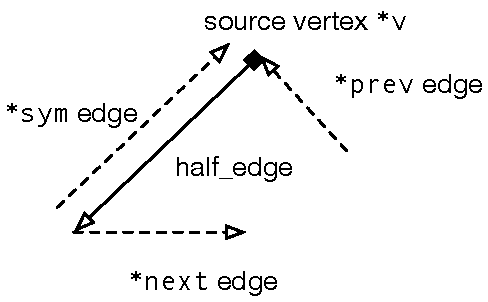
\includegraphics{figs/half_edge-data-structure}
\end{center}
\caption{Half Edge Data Structure}
\end{figure}


Our version of the half edge data structure is as follows:

\begin{verbatim}
    struct half_edge {
        int v; // index into the list of all vertices
        half_edge *prev, *next, *sym; // pointers to related edges
        edge_data* data; // bookkeeping for edge collapse
        int index; // bookkeeping for vertex splits
    };
\end{verbatim}

\section{Edge Collapses}

The task of collapsing an edge can be separated into several discrete sub-tasks. After finding the 
least-cost edge (see the section on Quadric Simplification, below, for details), we find the neighboring
edges that share a vertex with either end of the edge to be collapsed. We compute the new vertex for
the two ends of the collapsed edge, then update the \verb`half_edge`s surrounding the new vertex
to ensure the consistency of mesh.

\begin{figure}[htb]
  \begin{center}
    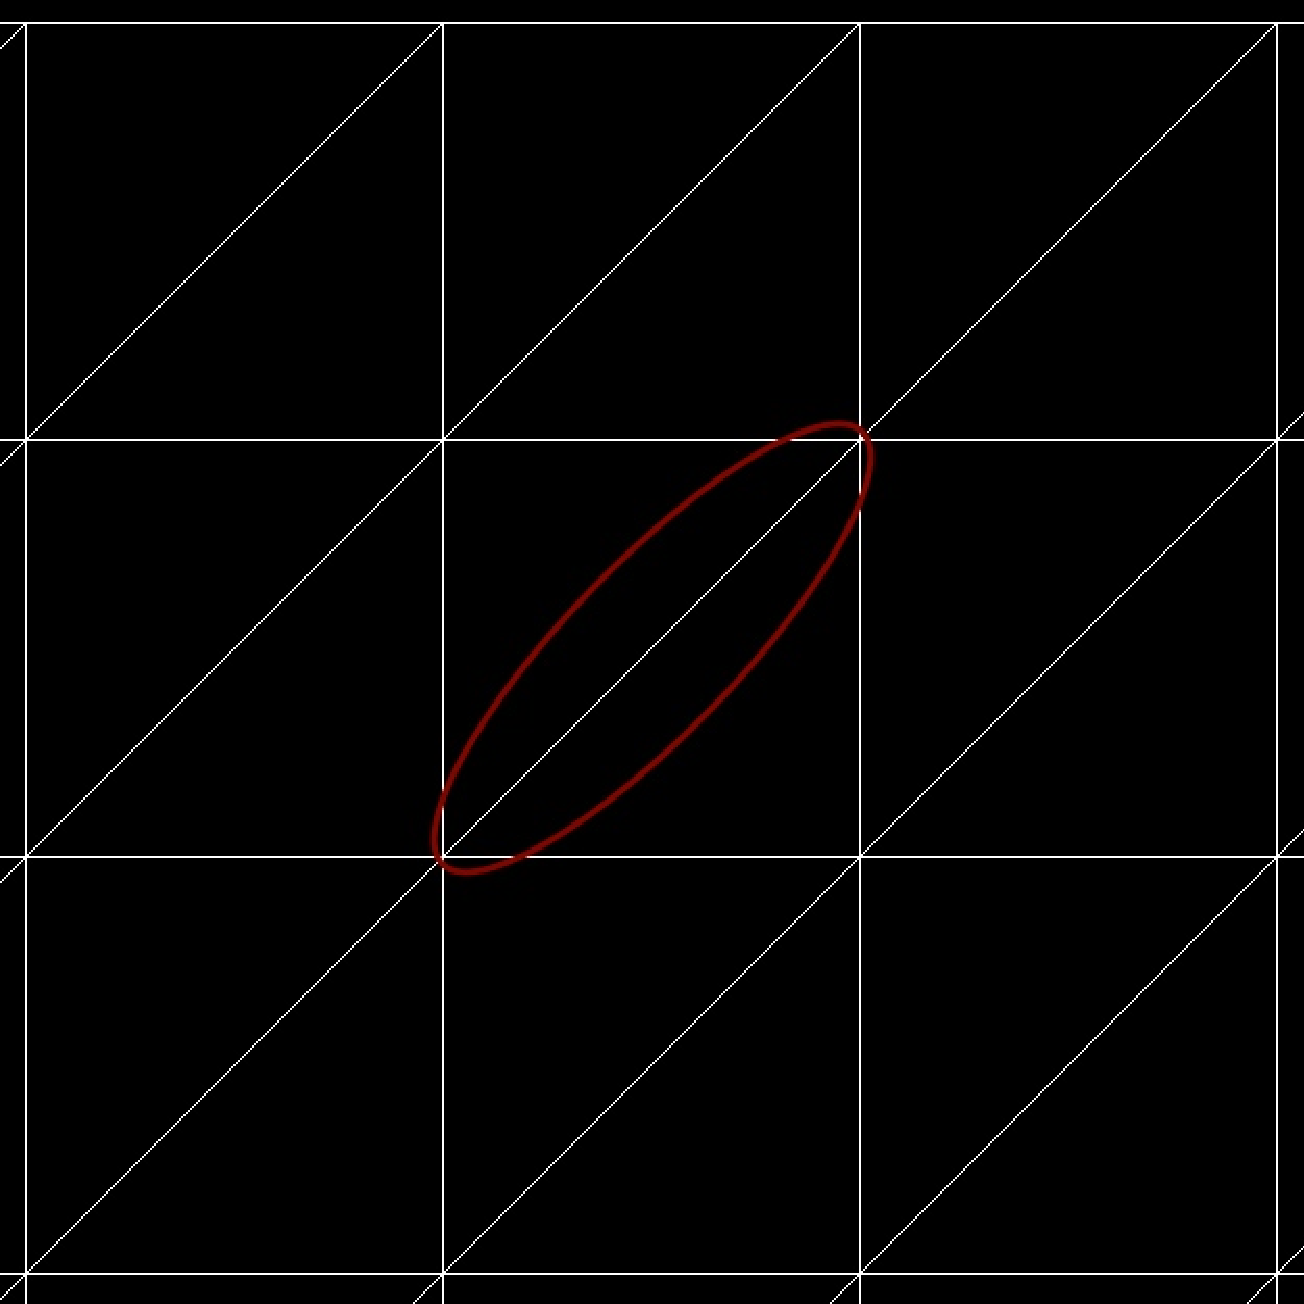
\includegraphics[width=.32\linewidth]{figs/ec1.pdf}
    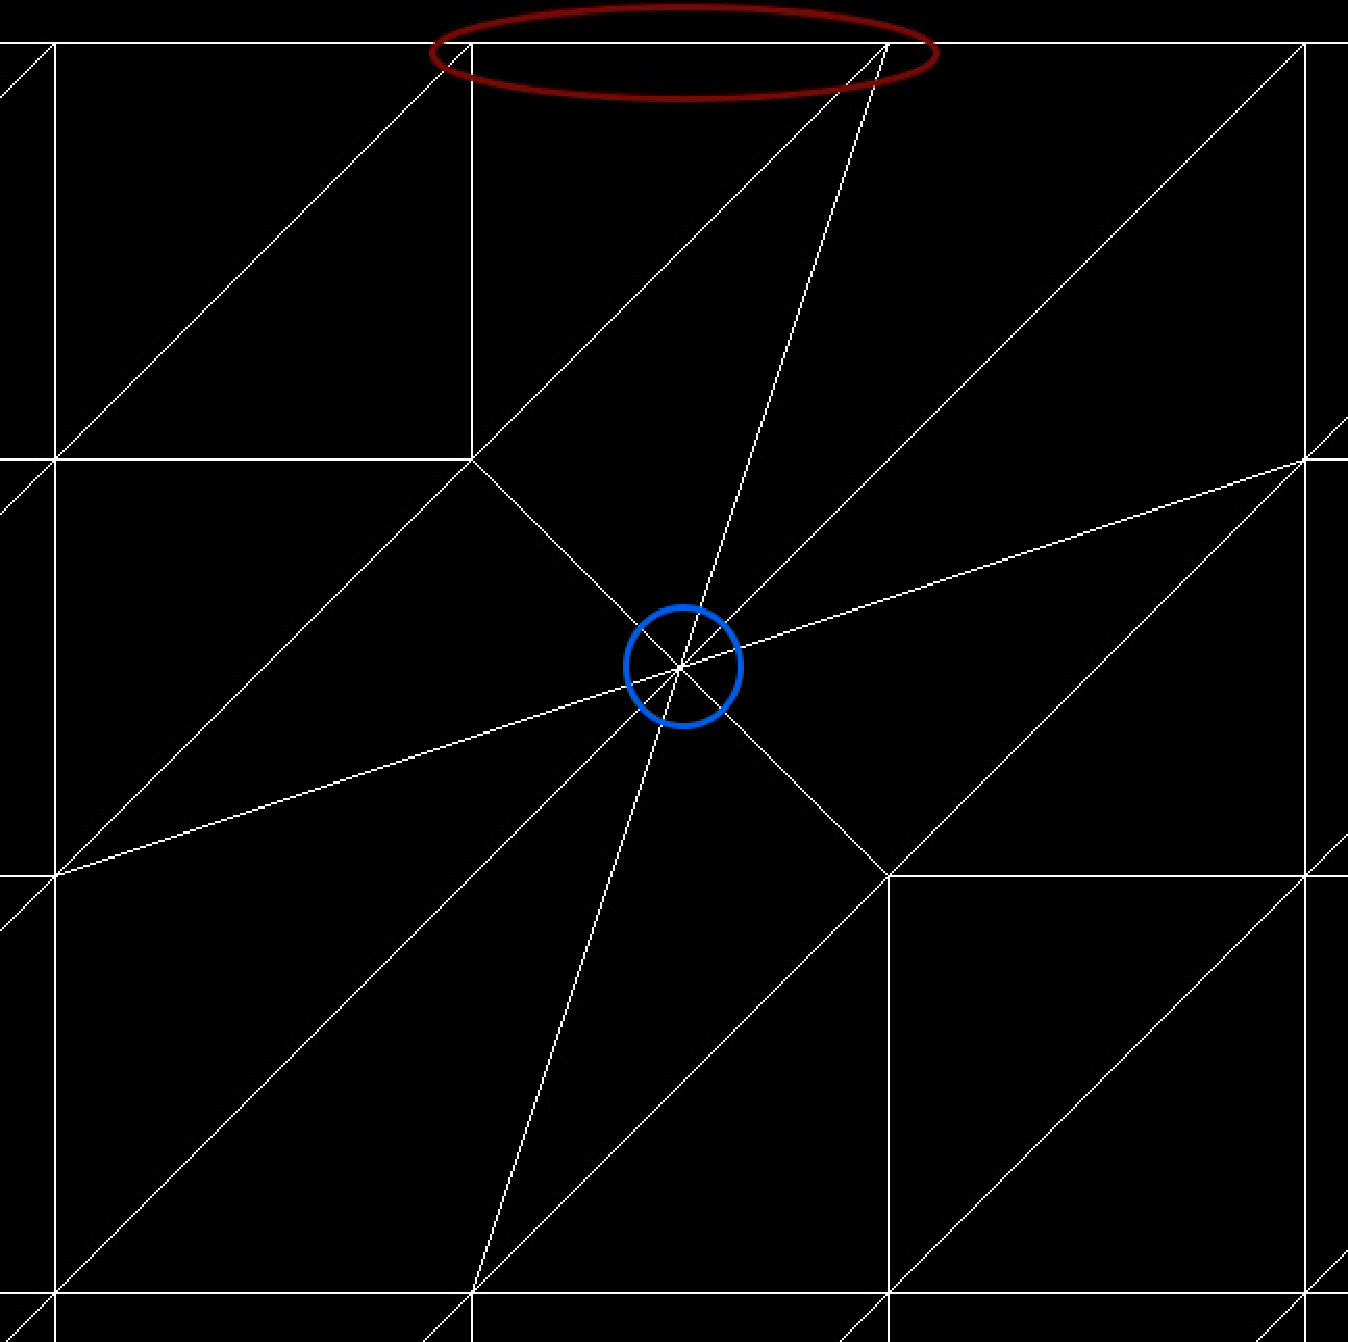
\includegraphics[width=.32\linewidth]{figs/ec2.pdf}
    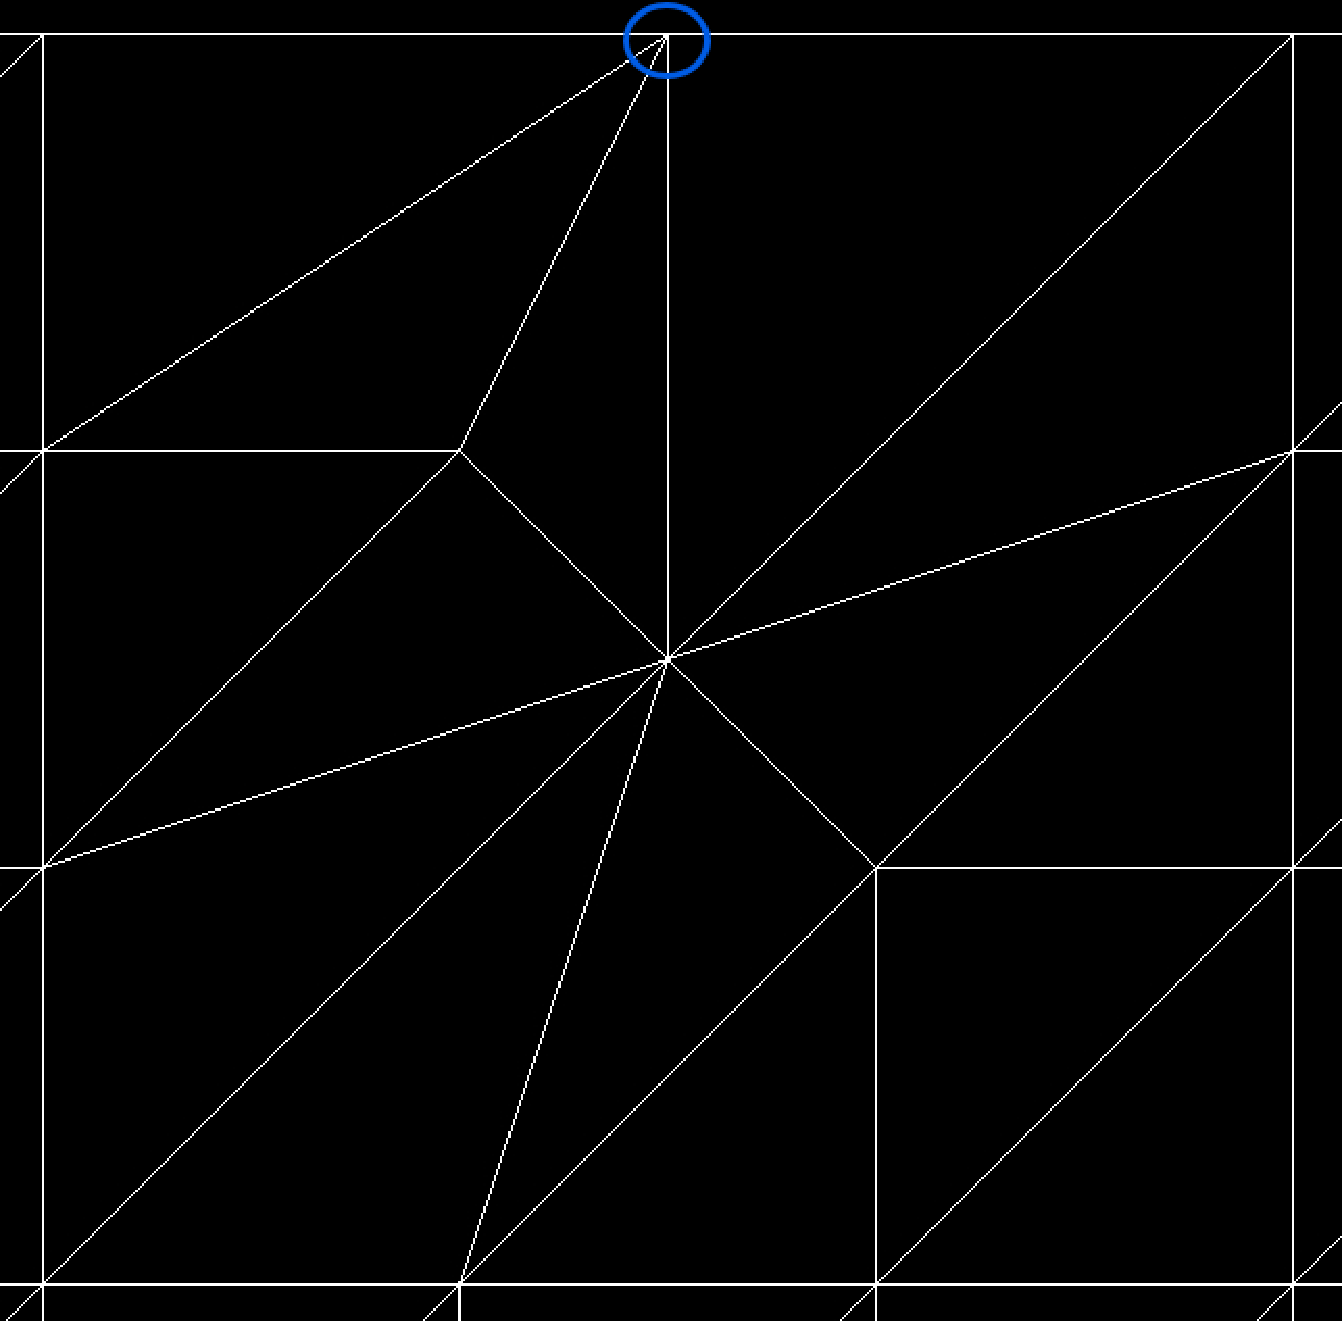
\includegraphics[width=.32\linewidth]{figs/ec3.pdf}
  \end{center}
\caption{Two successive edge collapses. The edge collapse is circled in red, and the resulting vertex
is circuled in blue. Here, we can see an example of collapsing a fully surrounded edge followed by
an example of collapsing a bordering edge.}
\end{figure}

\subsection{Finding Neighboring Edges}



\subsection{Updating Edge Pointers}
% go ahead and work here

\section{Quadric Simplification}

Every vertex has 10 floats that represent the quadric Q matrix. For every edge
in the mesh, an \verb`edge_data` object is created (one for every pair of symmetric
edges) which stores the optimum merge point for the two vertices and the
associated the quadric error. These objects are then stored in a priority queue
sorted by their quadric error. A handle to each of the objects in the in the
priority queue is stored with the associated edge, so that modified edges can
update their \verb`edge_data` object when the error is changed. To go down a level
of detail, the edge at the top of the priority queue is collapsed, and and
degenerate edges are removed from the queue.

\section{Progressive Meshes}

Objects are drawn using Vertex Buffer Objects (VBOs). After parsing all of the
vertices from the OFF file, new vertices are appended to the end of the vertex
when created during an edge collapse. This way, once all of the edges are
collapsed, we have calculated and stored all of vertices that are possible at
any level of detail. This makes switching between levels of detail very easy by
simply changing the indices in the element array buffer. This allows us to
simply store the changes in the indices for each level of detail. This is
implemented using a vector of \verb`collapse_data` objects which store the changes
need to move both up and down a level of detail.

\end{document}
